% author: Tomas Trnka
% mail: tomas@trnkatomas.eu
% date: 2013-07-04

\documentclass[a4paper,10pt]{article}
%\usepackage[czech]{babel}
%\usepackage[T1]{fontenc}
\usepackage[hmargin=2.2cm,vmargin=2.2cm]{geometry}
\usepackage[utf8x]{inputenc}
\usepackage{fancyhdr}
\usepackage{amsmath} 
\usepackage{amssymb} 
\usepackage{dsfont}
\usepackage{hyperref}
\usepackage{algpseudocode}
\usepackage{tikz}
\usetikzlibrary{patterns}
\usetikzlibrary{calc}
\usepackage{enumerate}
\pagestyle{fancy}
\headheight 15pt
\lhead{Crpyto, Fall 2014}
\rhead{Tomas Trnka}
\begin{document}
\section*{Exercise 11}
In the first step I rewrote the transformations in a table to visualise them in a readable way. It was necessary for me, to see what are the actual inputs for MAC.

\begin{table}[h!]
\centering
\begin{tabular}{|c|c|c|}
\hline 
input & padded &MAC tag \\ 
\hline 
$b$ & $b||1$ & $t_b$ \\ 
\hline 
$b' $& $b'||1 $& $t_{b'} $\\ 
\hline 
$b||1||c$ & $b||1||c $& $t_{b1c}$ \\ 
\hline 
$b||1||(t_b \oplus t_{b'} \oplus c)$ & $b||1||(t_b \oplus t_{b'} \oplus c)$ & $t_{b1c}$ \\ 
\hline
\end{tabular} 
\end{table}

Now plot the CBC-MAC scheme, this will help us to orientate during the process of creating MAC.
\begin{figure}[h!]
\centering
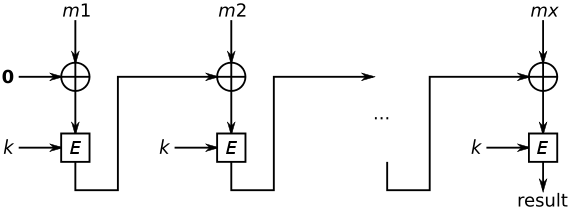
\includegraphics[scale=0.5]{CBC-MAC.png}
\end{figure}

Let's show that $t_{b1c}$ is a valid tag for the message $b||1||(t_b \oplus t_{b'} \oplus c)$
\begin{enumerate}[I.]
\item When we input the $b||1||(t_b \oplus t_{b'} \oplus c)$, the first part of the message is just $b$, while xor-ing with 0 nothing happens, and afterwards we will apply the hash function $E$.
\item In the next step we do xor with the second block, which in our case is $1$ and again encode. But what we have done so far is the same procedure how the $t_{b'}$ was created! So we can consider the input for the xor with next part of the message as $t_{b'}$.
\item In the next step will take a closer look at the xor with the next block:
$$
t_{b'} \oplus (t_b \oplus t_{b'} \oplus c)
$$
But when xor-ing bit string with itself we obtain zeros which does not change anything while applying the rest of the xors. After simplifying the expression the result will be.
$$
t_b \oplus c
$$
\item In the next step we have to encode this result of the last xor operation. But the input for this step is the same as we would have obtained after the second step of creating MAC for $t_{b1c}$, ie. we would have had the $t_b$ after MACing $b||1$ and the last part of the message would have been $c$. So we have shown that the tag for $b||1||c$ will be also valid for our forged message $b||1||(t_b \oplus t_{b'} \oplus c)$.
\end{enumerate}
\end{document}